\documentclass[10pt]{article}
\usepackage[margin=1in, paperwidth=8.5in, paperheight=11in]{geometry}
\usepackage{ifpdf,amsmath, amssymb, comment, color, graphicx, stmaryrd,setspace,enumitem,tikz, fancyhdr, wrapfig, textcomp, units, mathptmx, siunitx, pdfpages}
\usepackage{tikz}
\usepackage[colorlinks]{hyperref}
\usetikzlibrary{trees}

\setlength{\headheight}{14.5pt}
\newcommand{\Q}{\mathbb{Q}}
\newcommand{\R}{\mathbb{R}}
\newcommand{\Z}{\mathbb{Z}}
\newcommand{\vu}{\mathbf{u}}
\newcommand{\vv}{\mathbf{v}}
\newcommand{\vw}{\mathbf{w}}
\newcommand{\vi}{\mathbf{i}}
\newcommand{\vj}{\mathbf{j}}
\newcommand{\vk}{\mathbf{k}}
\newcommand{\vn}{\mathbf{n}}
\newcommand{\vr}{\mathbf{r}}
\newcommand{\va}{\mathbf{a}}
\newcommand{\vF}{\mathbf{F}}
\newcommand{\vL}{\mathbf{L}}
\newcommand{\vT}{\mathbf{T}}
\newcommand{\vN}{\mathbf{N}}
\newcommand{\proj}{\operatorname{proj}}
\newcommand{\orth}{\operatorname{orth}}
\newcommand\del\nabla
\newcommand\dotp[1][.5]{\,\mathbin{\vcenter{\hbox{\scalebox{#1}{$\bullet$}}}}\,}

% Solution text is in red. If you want the solutions to show, remove the \iffalse from the definition of the \red command.
%\newcommand{\red}[1]{ %\iffalse
%	\textcolor{red}{#1} }%\fi}

\newenvironment{red}{\color{red}}{\ignorespacesafterend}
\newcommand{\blue}[1]{\textcolor{blue}{#1}}
\newcommand{\green}[1]{\textcolor{green}{#1}}
\renewcommand{\section}[1]{\begin{center} \textbf{#1} \\\end{center}}
%
\hyphenpenalty=5000
\setlength{\parindent}{0in}
%\oddsidemargin=-.25in
\allowdisplaybreaks
\pagestyle{fancy}
\renewcommand{\headrulewidth}{0pt}
\lhead{MATH 203}
\rhead{Spring 2020}
%\lfoot{\copyright\ CLEAR Calculus 2010}
\cfoot{}

\begin{document}
%


%\onehalfspacing
\allowdisplaybreaks
%##################################################################
\section{PS\#9: Optimization and Lagrange multipliers  - \red{Answer key} }

\begin{enumerate}[leftmargin=0pt]
\item (AC Multi 10.8 Exercise 12) The Cobb-Douglas production function is used in economics to model production levels based on labor and equipment. Suppose we have a specific Cobb-Douglas function of the form \[f(x, y) = 50 x^{0.4}y^{0.6},\] where $x$ is the dollar amount spent on labor and $y$ the dollar amount spent on equipment. Use the method of Lagrange multipliers to determine how much should be spent on labor and how much on equipment to maximize productivity if we have a total of \$1.5 million dollars to invest in labor and equipment.
    
\begin{red}
The method of Lagrange multipliers needs us to have a constraint. Here the constraint is the total amount of money:
\[x + y = 1.5 \textrm{ million}.\]
So, our $f$ is the function given in the problem, our $g(x,y) = x+y = 1.5$. Off we go to Lagrange mulitpliers land. We need to calculate the gradients: 
\begin{align*}
    \del f &= \langle 20 x^{-0.6} y^{0.6}, 30 x^{0.4} y^{-0.4} \rangle \\
    \del g &= \langle 1, 1 \rangle
    \intertext{So, setting up $\del f = \lambda \del g$ together with our constraint:}
    20 x^{-0.6} y^{0.6} &= \lambda\cdot 1 \\
    30 x^{0.4} y^{-0.4} &= \lambda\cdot 1 \\
    x+y &= 1.5
    \intertext{It's nice that we have two things that both equal $\lambda$, so they must just equal each other. Also, our constraint tells us that $y=1.5-x$:}
    20 x^{-0.6} (1.5-x)^{0.6} &= 30 x^{0.4} (1.5-x)^{-0.4} \\
    20\frac{(1.5-x)^{0.6}}{x^{0.6}} &= 30 \frac{x^{0.4}}{(1.5-x)^{0.4}}
    \intertext{Clear denominators. It's so nice that the powers add up to 1, eh?}
    20 (1.5-x)^{0.6} (1.5-x)^{0.4} &= 30 x^{0.4} x^{0.6} \\
    20 (1.5-x) &= 30 x \\
    30 - 20x &= 30x \\
    30 &= 50x \\
    x = 0.6; &\quad y = 0.9
\end{align*}
So we should spend $\$600,000$ on labor and $\$900,000$ on equipment.
\end{red}


\item (AC Multi 10.8 Exercise 14c) Find the absolute maximum and minimum of $f(x,y,z) = x^2+y^2+z^2$ subject to the constraint that $(x-3)^2 + (y+2)^2 + (z-5)^2 \le 16\text{.}$ (Hint: here the constraint is a closed, bounded region. Use the boundary of that region for applying Lagrange Multipliers, but don't forget to also test any critical values of the function that lie in the interior of the region.)

\begin{red}
Let's do the easy part first and check for critical points inside the region. Since $\del f = \langle 2x, 2y, 2z \rangle$, the only critical point is $(0, 0, 0)$. This isn't inside the region because $(0-3)^2 + (0+2)^2 + (0-5)^2 = 9 + 4 + 25 = 38$, which is certainly bigger than 16. So we can ignore that critical point; any maxes or mins in this situation will occur on the boundary.

Let's set up our Lagrange multiplier equations $\del f = \lambda \del g$ together with the constraint:
\begin{align*}
    2x &= \lambda\cdot 2(x-3) \\
    2y &= \lambda \cdot 2(y+2) \\
    2z &= \lambda \cdot 2(z-5) \\
    (x-3)^2 &+ (y+2)^2 + (z-5)^2 = 16
\end{align*}
I'm going to ask W$|$A to solve this system of equations so I can skip a lot of tedious algebra. Here's the result (I used $L$ for $\lambda$ because I can't type $\lambda$ into W$|$A):

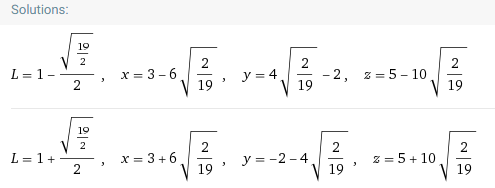
\includegraphics[]{203-keys/ps9-answer-key/wa-exact.png}

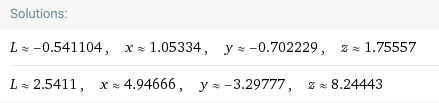
\includegraphics[]{203-keys/ps9-answer-key/wa-approx.png}

One of these is going to give us a min and the other will give us the max. To tell which is which, we just need to feed our points into $f(x,y,z)$:
\begin{align*}
    f(1.05334, -0.702229, 1.75557) &= 4.68468 \\
    f(4.94666, -3.29777, 8.24443) &= 103.315
\end{align*}

Cool, so the first point definitely is the location of the minimum, and the second is definitely the location of the maximum.

(By the way, a geometric interpretation of this problem: $f(x,y,z)$ is the square of the distance from your point $(x,y,z)$ to the origin, and the region is a sphere centered at $(3, -2, 5)$ with radius 4, together with the inside of the sphere. So you're looking for the minimum and maximum (square of the) distance from the sphere to the origin. Since the origin isn't actually inside this sphere (check!), it makes sense that both the min and the max are on the boundary. You can even check that these two points are ``antipodal.'')
\end{red}

\end{enumerate}
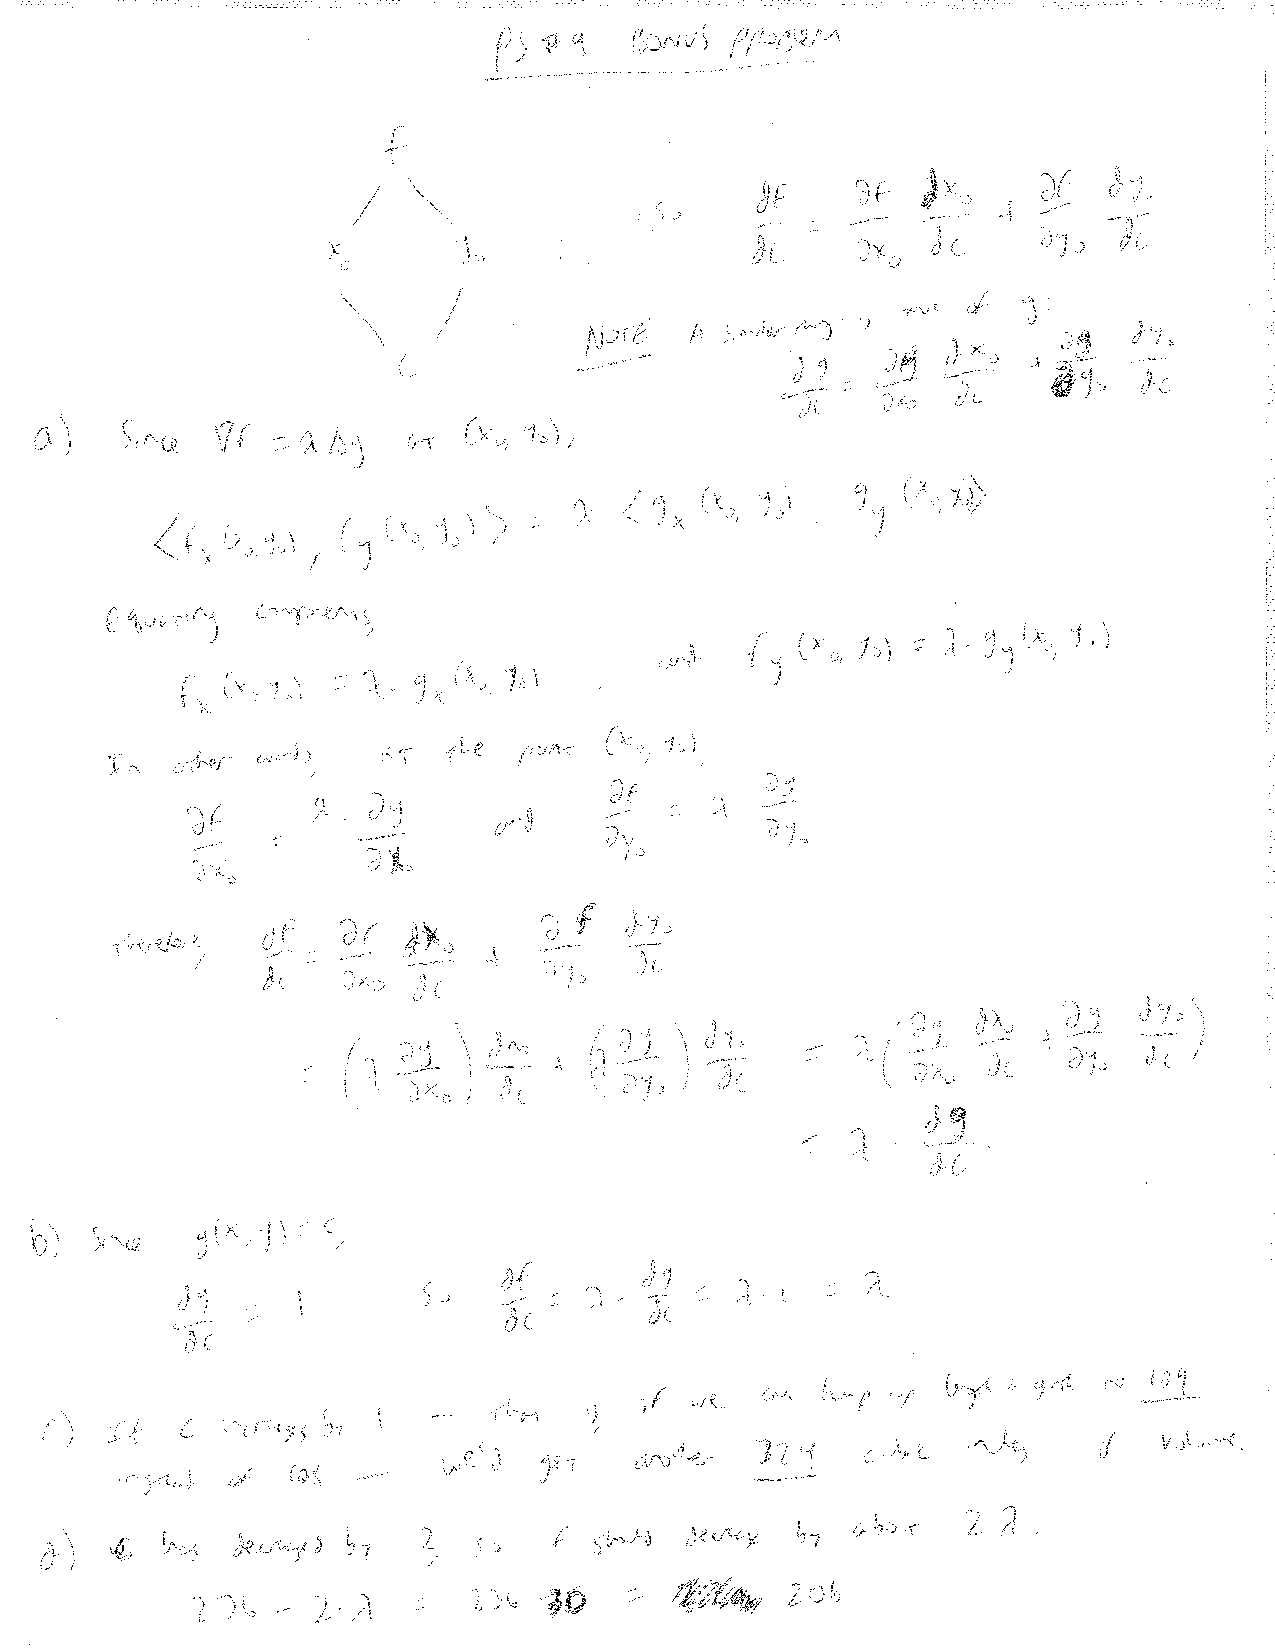
\includepdf[pages=-]{ps-9-bonus.pdf}
\end{document}